\documentclass[border=8pt]{standalone}
\usepackage[utf8]{inputenc}
\usepackage{tikz}
\tikzset{
  entita/.style = {rectangle, draw, thick, fill=blue!8, minimum width=32mm, minimum height=16mm, font=\small},
  attr/.style   = {circle, draw, thick, fill=white, minimum size=5pt, inner sep=0},
  pk/.style     = {circle, draw, thick, fill=black, minimum size=5pt, inner sep=0},
  link/.style   = {thick}, et/.style = {font=\footnotesize}
}
\begin{document}
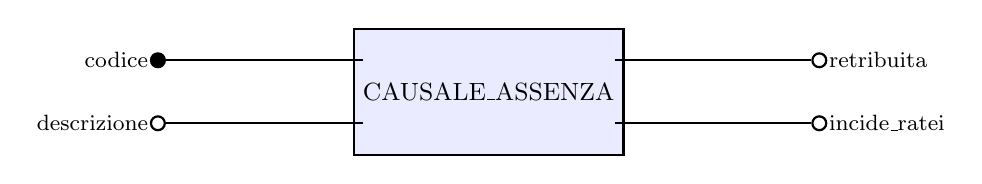
\begin{tikzpicture}
  \node[entita] (E) {CAUSALE\_ASSENZA};
  \node[pk]   (c) at (-4.2, 0.4){}; \draw[link] (-1.6, 0.4)--(c); \node[et,left] at (c) {codice};
  \node[attr] (d) at (-4.2,-0.4){}; \draw[link] (-1.6,-0.4)--(d); \node[et,left] at (d) {descrizione};
  \node[attr] (r) at ( 4.2, 0.4){}; \draw[link] ( 1.6, 0.4)--(r); \node[et,right] at (r) {retribuita};
  \node[attr] (ir) at ( 4.2,-0.4){}; \draw[link] ( 1.6,-0.4)--(ir); \node[et,right] at (ir) {incide\_ratei};
\end{tikzpicture}
\end{document}
